\documentclass[13pt]{beamer}
\usetheme{CambridgeUS}
\usecolortheme{dolphin}

\usepackage{microtype}
\usepackage{amsmath}
\usepackage{lmodern}
\usepackage{tikz}
\usepackage[czech,slovak]{babel}
\usepackage[utf8x]{inputenc}
\usepackage{times}
\usepackage{pgfpages}
\usepackage{amssymb}
\usepackage{graphicx}
\usepackage{listings}
\usepackage{palatino}

\setbeamertemplate{note page}{\pagecolor{yellow!5}\insertnote}

\usetikzlibrary{calc,trees,positioning,arrows,chains,shapes.geometric,%
    decorations.pathreplacing,decorations.pathmorphing,shapes,%
    matrix,shapes.symbols}

\title{Interpret jazyka IFJ16 (a/4/I)}
\subtitle{Semestrální projekt IFJ}
\institute{FIT VUT Brno}
\author[ Tamaškovič,Vaško,Vaško,Záleský,Zárybnický]
{Marek~Tamaškovič,Martin~Vaško, Michal~Vaško, Jiří~Záleský, Jakub~Zárybnický}
\date{14. prosince 2016}

\newsavebox{\grammarbox}

\begin{document}

\begin{frame}
  \titlepage
  \note[item]{Varianta a/4/I - Knuth–Morris–Pratt algoritmus pre vyhledáni podřetezce v řetezci, jako seřaďovací algoritmus byl použit List-Merge a tabulka symbolu byla implementovaná pomoci BVS.}
\end{frame}

\section{Úvod}

\subsection{Zadání}

\section{Architektura}

\begin{frame}{Přehled architektury}
\begin{center}
\begin{tikzpicture}
[node distance = 1cm, auto,,
every node/.style={node distance=2cm},
force/.style={rectangle, rounded corners, draw=black, very thick,
text width=8em, text badly centered, minimum height=3em}]

% Draw forces
\node [force] (center) {Hlavní řadič};
\node [force, left=.5cm of center] (database) {Databáze};
\node [force, below=.5cm of center] (gui) {Grafické rozhraní};
\node [force, below=.5cm of gui] (user) {Uživatel};
\node [force, right=.5cm of center] (server) {Server};

\path[->,thick,shorten >=1pt,shorten <=1pt]
(center) edge (database)
(center) edge (gui)
(center) edge (server)
(gui) edge (center)
(server) edge (center)
(database) edge (center)
(user) edge (gui)
(gui) edge (user);

\end{tikzpicture}
\end{center}
\end{frame}

\begin{frame}{Datové typy (AST)}
\end{frame}

\begin{frame}{Hierarchie typů}
\end{frame}

\section{Komponenty}
\subsection{Lexer}

\begin{frame}{Poznámky k implementaci (změnit název?)}
počítání line, char, BASE
\end{frame}

\begin{frame}{Stavový diagram lexeru}
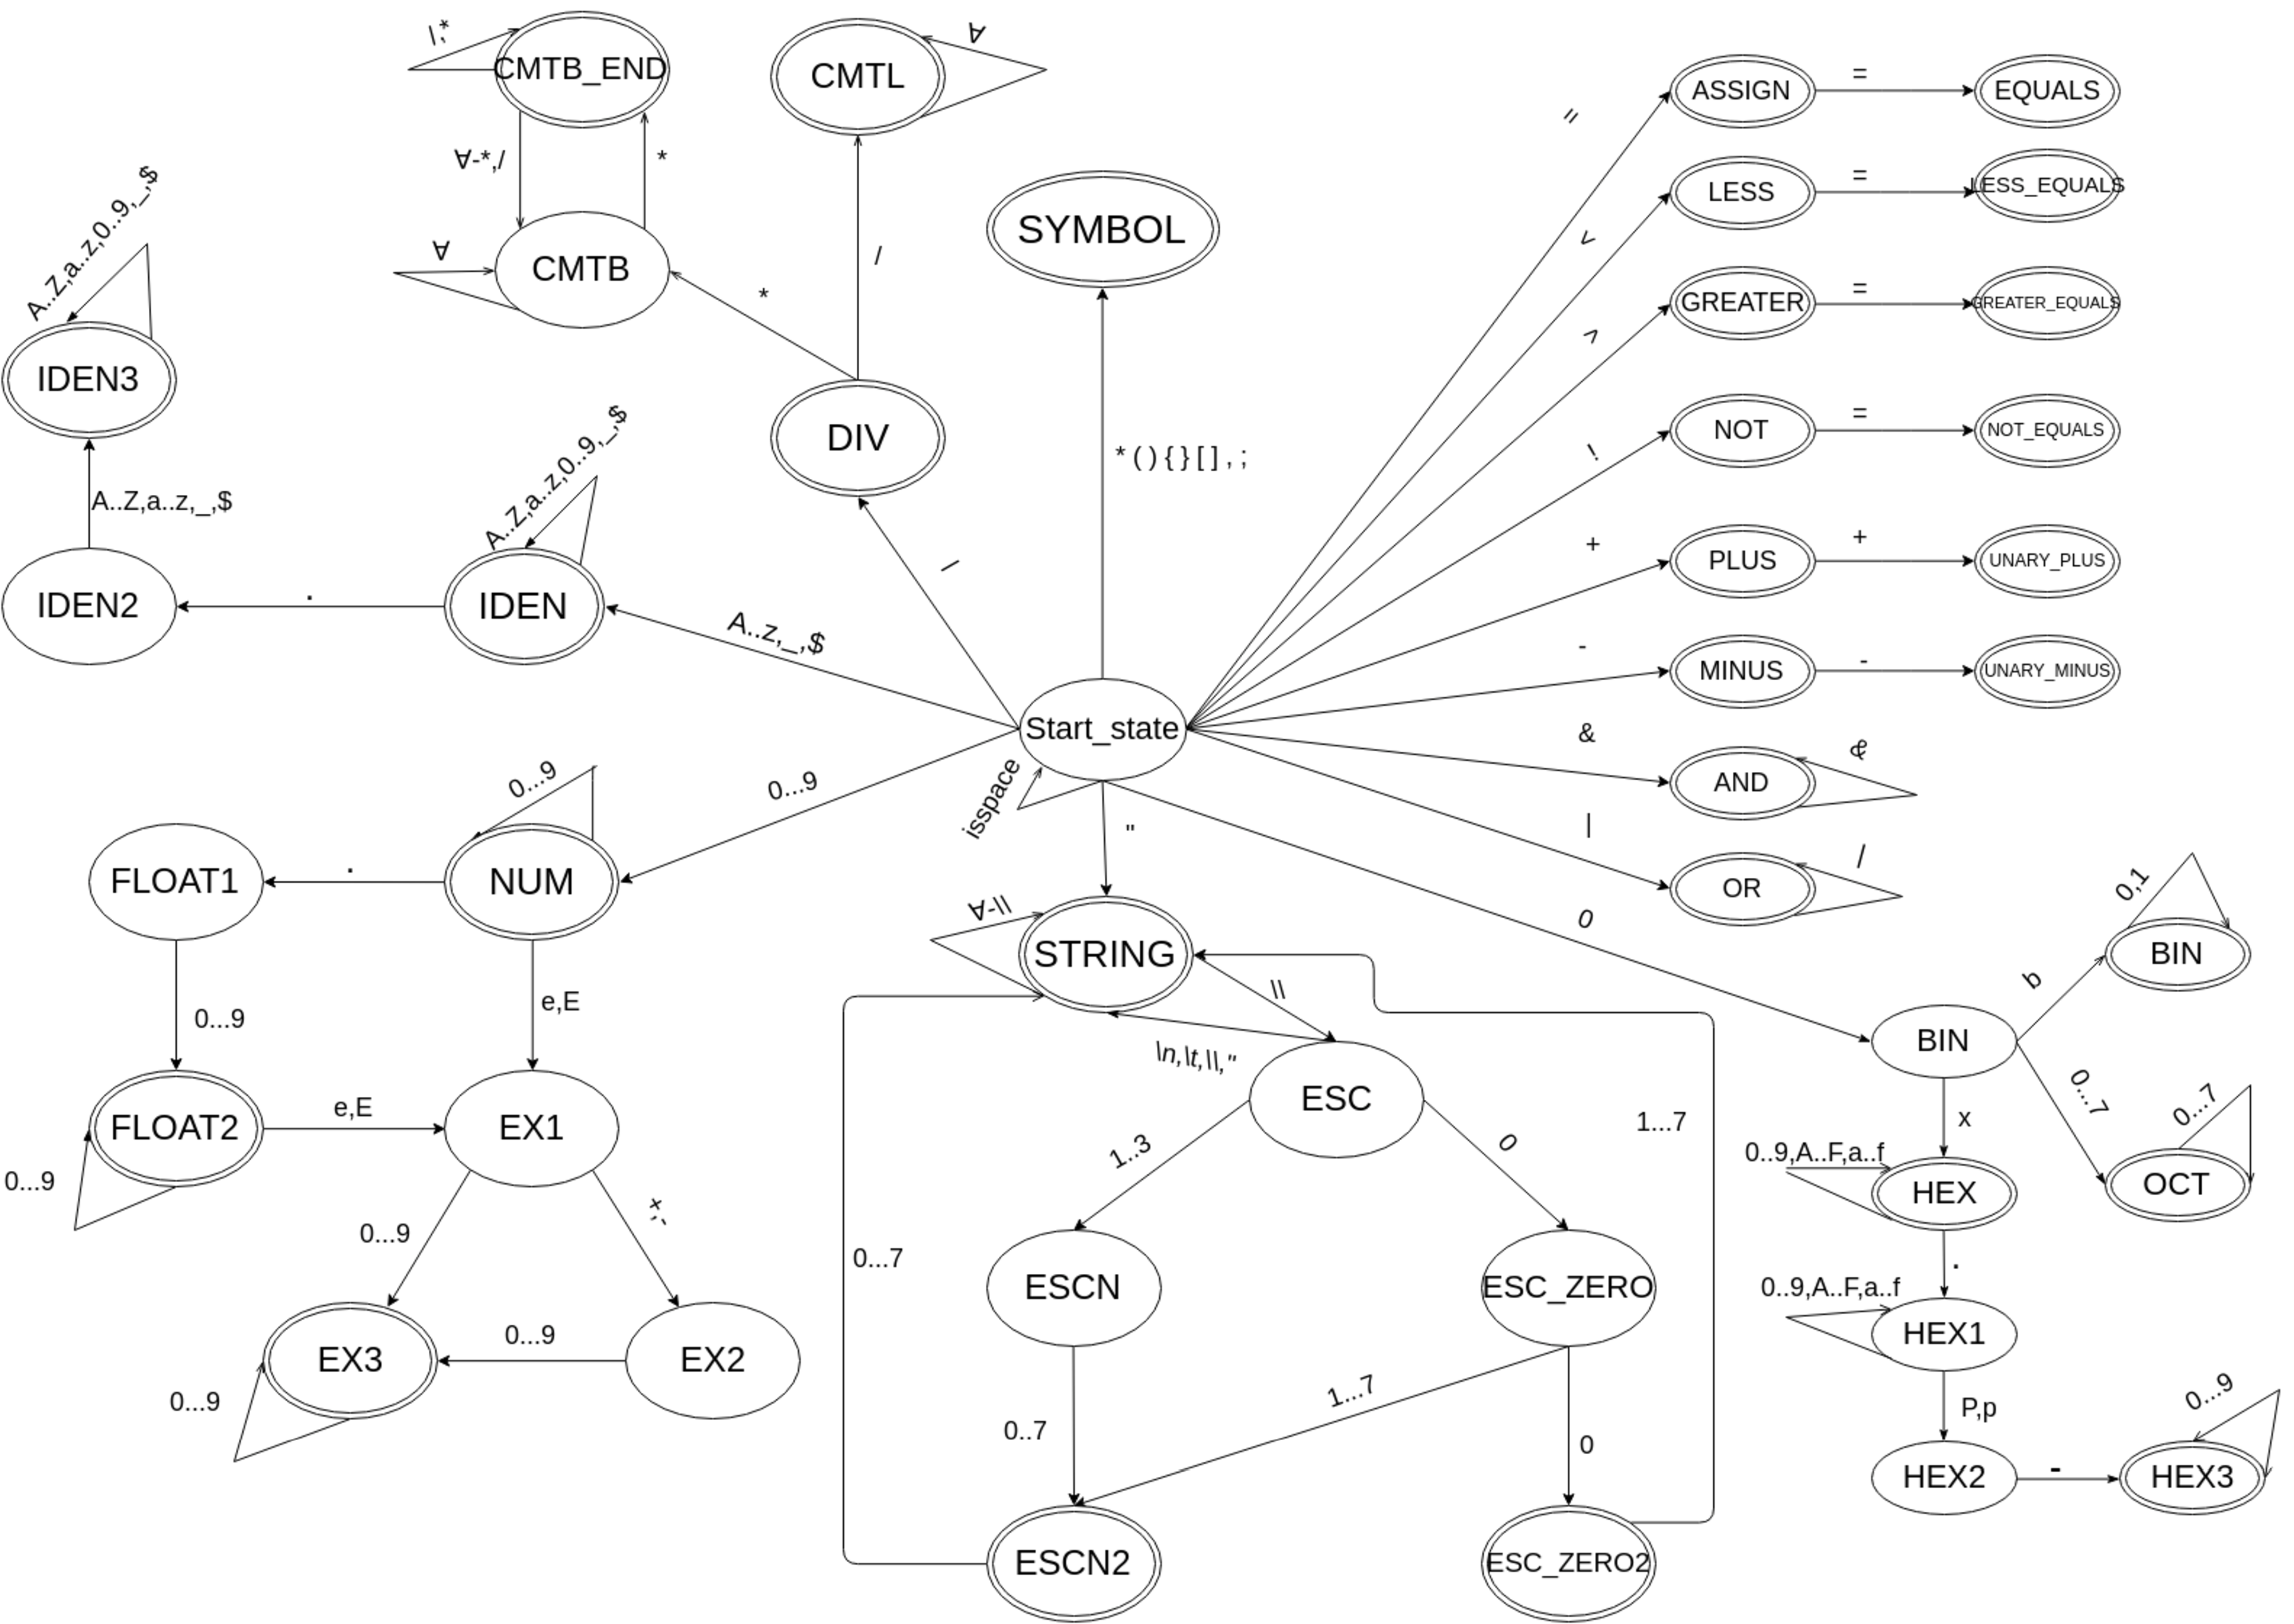
\includegraphics[width=0.9\textwidth]{./img/lex1.pdf}
% \begin{center}
% \begin{tikzpicture}
%    [>=stealth',
%    punktchain/.style={
%      rectangle,
%      rounded corners,
%      draw=black, very thick,
%      text width=10em,
%      minimum height=2.5em,
%      text centered,
%     on chain},
%    every join/.style={->, thick,shorten >=1pt},
%    \node distance=.5cm, start chain=going below,]
%    \node[punktchain, join] {Anal\'yza};
%    \node[punktchain, join] {Návrh};
%    \node[punktchain, join] {Implementace};
%    \node[punktchain, join] {Testov\'an\'i};
%    \node[punktchain, join] {Publikování};
%  \end{tikzpicture}
%  \end{center}

\end{frame}

\subsection{Parser}

\begin{frame}{Poznámky k implementaci (změnit název?)}
UNARY, re-re-re-implemeentace, makra
\end{frame}

\begin{frame}[fragile]{LL gramatika}
\begin{lrbox}{\grammarbox}%
    \begin{lstlisting}%
ifj16 = \$ | class ifj16
class = "class" "{" classBody
classBody = "}" | "static" type simpleId classBody'
classBody' = ";"
           | "=" expression ";"
           | "(" declarationList "{" functionBody
functionBody = "}"
              | type simpleId(q) functionBody'
              | command
functionBody' = ";" | "=" expression ";"
command = "if" "(" expression ")" command
        | "while" "(" expression ")" command
        | "do" command "while" "(" expression ")" ";"
        | "for" "(" type simpleId for'
        | "return" return'
        | "{" commandList
        | "break" ";"
        | "continue" ";"
        | anyId command'
for' = ";" for'' | "=" expression ";" for''
for'' = expression ";" anyId "=" expression ")" command
return' = ";" | expression ";"
commandList = "}" | command commandList
command' = "(" argumentList ";" | "=" expression ";"
declarationList  = ")" | type simpleId declarationList'
declarationList' = ")" | "," type simpleId declarationList'
argumentList  = ")" | expression argumentList'
argumentList' = ")" | "," expression argumentList'
type = "int" | "double" | "boolean" | "String" | "void"
anyId = simpleId | compoundId
    \end{lstlisting}%
\end{lrbox}%
\scalebox{0.52}{\usebox{\grammarbox}}
\end{frame}

\begin{frame}{Precedenční tabulka}
\scalebox{0.55}{
\begin{tabular}[pos]{r|l|l|l|l|l|l|l|l|l|l|l|l|l|l|l|l|l|l|l|l|l|l|l}
    &(&)&++&--&u-& !& *& /& +& -& <& >&<=&>=&==&!=&\&\&&$\|$&id&li&tf&,& \$ \\
    (& L& E& L& L& L& L& L& L& L& L& L& L& L& L& L& L& L& L& L& L& L& E& O \\
    )& O& G& O& O& O& O& G& G& G& G& G& G& G& G& G& G& G& G& O& O& O& G& G \\
    ++& O& G& G& G& O& O& G& G& G& G& G& G& G& G& G& G& G& G& L& O& O& G& G \\
    --& O& G& G& G& O& O& G& G& G& G& G& G& G& G& G& G& G& G& L& O& O& G& G \\
    u-& L& G& O& O& G& G& G& G& G& G& G& G& G& G& G& G& G& G& L& G& L& O& G \\
    !& L& G& O& O& G& G& G& G& G& G& G& G& G& G& G& G& G& G& L& G& L& O& G \\
    *& L& G& L& L& L& L& G& G& G& G& G& G& G& G& G& G& G& G& L& L& L& G& G \\
    /& L& G& L& L& L& L& G& G& G& G& G& G& G& G& G& G& G& G& L& L& L& G& G \\
    +& L& G& L& L& L& L& L& L& G& G& G& G& G& G& G& G& G& G& L& L& L& G& G \\
    -& L& G& L& L& L& L& L& L& G& G& G& G& G& G& G& G& G& G& L& L& L& G& G \\
    <& L& G& L& L& L& L& L& L& L& L& G& G& G& G& G& G& G& G& L& L& L& G& G \\
    >& L& G& L& L& L& L& L& L& L& L& G& G& G& G& G& G& G& G& L& L& L& G& G \\
    <=& L& G& L& L& L& L& L& L& L& L& G& G& G& G& G& G& G& G& L& L& L& G& G \\
    >=& L& G& L& L& L& L& L& L& L& L& G& G& G& G& G& G& G& G& L& L& L& G& G \\
    ==& L& G& L& L& L& L& L& L& L& L& L& L& L& L& G& G& G& G& L& L& L& G& G \\
    !=& L& G& L& L& L& L& L& L& L& L& L& L& L& L& G& G& G& G& L& L& L& G& G \\
    \&\&& L& G& L& L& L& L& L& L& L& L& L& L& L& L& L& L& G& G& L& L& L& G& G \\
    $\|$& L& G& L& L& L& L& L& L& L& L& L& L& L& L& L& L& L& G& L& L& L& G& G \\
    id& E& G& G& G& O& O& G& G& G& G& G& G& G& G& G& G& G& G& O& O& O& G& G \\
    literal& O& G& O& O& O& O& G& G& G& G& G& G& G& G& G& G& G& G& O& O& O& G& G \\
    true/false& O& G& O& O& O& O& G& G& G& G& G& G& G& G& G& G& G& G& O& O& O& G& G \\
    ,& L& E& L& L& L& L& L& L& L& L& L& L& L& L& L& L& L& L& L& L& L& E& O \\
    \$& L& O& L& L& L& L& L& L& L& L& L& L& L& L& L& L& L& L& L& L& L& O& O
\end{tabular}
}
\end{frame}

\subsection{Sémantická analýza}

\begin{frame}{Zaujimavosti v implementácii ???}
  \begin{itemize}
    \item V projekte používame funkcionálné programovanie.
    \item Nachádzajú sa tam rôzne kontroly napr.: \texttt{getExpressionType, isAssignCompatible}
  \end{itemize}
\end{frame}

\subsection{Interpret}

\begin{frame}{Poznámky k implementaci (změnit název?)}

\note[item]{Doslovný přepis cyklů - for v ifj16 je for v C apod.}

  \begin{itemize}
    \item Makra opět tvoří velkou část kódu
    \item \texttt{\#define I(x) (x)->data.integer}
    \item \texttt{I(result) = I(left) + I(right)}
    \item \texttt{CYCLE\_INNER(...)} (break, continue, return handling)
    \item \texttt{while (evalExpression(...)) \{ CYCLE\_INNER(...); \}}
    \item We didn't consider GOTO harmful (Dijkstra, 1968)
    \item Základní garbage collector (GC pouze při skončení)
  \end{itemize}

\end{frame}

\section{Vestavěné funkce + Algoritmy}

\begin{frame}{Vestavěné funkce + Algoritmy}

  \begin{itemize}
    \item Seřazení prvků v poli - List-Merge sort $\mathcal{O}(n log(n))$
    \item Najít podřetězec v řetězci - Knutt-Morris-Pratt $\mathcal{O}(n)$
    \item Tabulka symbolů - BVS - vyhledání $\mathcal{O}(log (n))$
  \end{itemize}
  \note[item] {Binární vyhledávací strom - základem je vkladání a nalezení uzlu, AVL strom sme se rozhodli vyvažovat z důvodu mnoha uzlů (hlavně vestavěné funkce), a tím pádem rychleji daný uzel najít. - spíše teoretické cvičení, na skutečnou rychlost nemá velký vliv}
\end{frame}

\section{Závěr}

\begin{frame}{Statistiky, očekávání, rozpočet a zhodnocení}
Ďekujeme za pozornost
\end{frame}

\end{document}
